\documentclass[12pt]{article}

\usepackage[utf8]{inputenc}
\usepackage[english]{babel}
\usepackage{natbib}
\usepackage[T1]{fontenc}
\usepackage{setspace}
\usepackage{graphicx}
\usepackage{hyperref}
\usepackage{float}
\usepackage[top=3.5cm,left=2.7cm,right=2.7cm,bottom=3.5cm]{geometry} % 'showframe' to see borders
\usepackage{booktabs}
\usepackage{subcaption}


\graphicspath{ {diagrams/} }

\title{\vspace{2cm}6G6Z1705\\\textbf{Artificial Intelligence}\\\vspace{2cm}Scenario 1\\\vspace{2cm}}
\author{14032908\\Joshua Michael Ephraim Bridge\\joshua.m.bridge@stu.mmu.ac.uk\\\vspace{1cm}}

\begin{document}

\maketitle

\newpage

% \doublespacing

\onehalfspacing

\section{Introduction}
In this report a process will be laid out which removes redundant parameters from images containing numeric digits. This includes reducing noise in the images and supplying information about the shapes. The data will then be input into WEKA to distinguish between the different digits.

\section{Image Processing Methods}
  Noise within images distracts from classification, therefore it is vital to remove as much of it as possible. Below are some methods which will be used to remove noise / stabilize the images as a pre-step for other image encoding methods (section \ref{encoding}).

  \subsection{Scaling}
    The first chosen method for improving image data is through scaling of the image. While this method does not remove noise from the image, it allows other image processing / encoding methods to have more data points - such as creating a chain code (section \ref{chain-code}).

  \subsection{Gaussian Blurring} \label{sec:gauss-blur}
    A popular method for reducing noise is gaussian smoothing. With this method a gaussian kernel is applied as a convolution to pixel data which thereby produces a blurring effect on the image. This reduces grain noise but can also reduce detail within the image therefore a small standard deviation is key to not removing too much detail. Figure \ref{fig:gauss-filter} shows a gaussian convolution applied to an image from the dataset with the gaussian standard deviation set to 1.

    \begin{figure}[H]
      \begin{subfigure}{.5\textwidth}
        \centering
        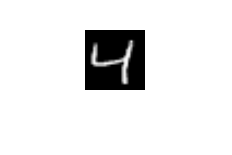
\includegraphics[width=0.5\textwidth]{scaled}
        \caption{Plain image}
        \label{fig:scaled}
      \end{subfigure}
      \begin{subfigure}{.5\textwidth}
        \centering
        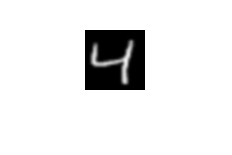
\includegraphics[width=0.5\textwidth]{blurred}
        \caption{Blurred image}
        \label{fig:blurred}
      \end{subfigure}
      \caption{Gaussian smoothing}
      \label{fig:gauss-filter}
    \end{figure}

  \subsection{Otsu thresholding} \label{otsu-thres}
    Creating a binary version of an image is a very useful tool for reducing noise. \cite{otsu1979threshold} presents a method which works by finding the threshold pixel value that minimises intra-class variance between black and white colours. Due to the removal of high variancy in pixel data it leaves a distinct binary shape which is much easier to extract shape information from, so long as there is not much noise in the image beforehand. An example of Otsu's method being applied to a gaussian blurred image can be seen in figure \ref{fig:otsu-threshold}. Applying the thresholding method on top of gaussian blurring ensures the resulting shape is smoother and has less noise around the shape edges.

    \begin{figure}[H]
      \begin{subfigure}{.5\textwidth}
        \centering
        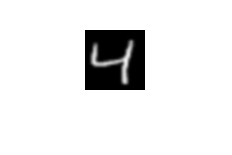
\includegraphics[width=0.5\textwidth]{blurred}
        \caption{Blurred image}
        \label{fig:blurred-2}
      \end{subfigure}
      \begin{subfigure}{.5\textwidth}
        \centering
        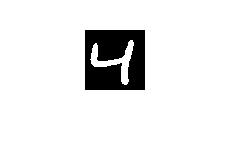
\includegraphics[width=0.5\textwidth]{ohtsu}
        \caption{Thresholded image}
        \label{fig:ohtsu}
      \end{subfigure}
      \caption{Otsu thresholding}
      \label{fig:otsu-threshold}
    \end{figure}

  \subsection{Image eroding (edge finding)} \label{eroded}
    Finding the edges of shapes is a useful tool when creating a chain code (section \ref{chain-code}). \cite{haralick1987image} show that a good way to manipulate shape data is via morphological processing. In this case it will be used to erode the shape's size using a little cross as a kernel, then subtracting the eroded shape from the original will leave a border around the shape's edges (illustrated in figure \ref{fig:eroded}). Note that this requires the image to be in binary form which will be done via Otsu thresholding (section \ref{otsu-thres}).

    \begin{figure}[H]
      \centering
      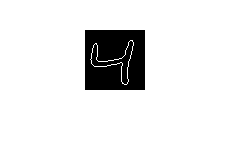
\includegraphics[width=0.25\linewidth]{edge}
      \caption{Shape edge after image erosion}
      \label{fig:eroded}
    \end{figure}

\section{Image Encoding methods} \label{encoding}
  Once as much noise / redundant information has been removed from the images as possible, it is then neccesary to exctract useful shape \& texture information which will aide the classifier in distinguishing between handwritten digits.

  \subsection{Chain Code} \label{chain-code}
   A chain code \citep{freeman1961encoding} is a very useful method for gathering shape information, especially for easily defined shapes such as handwritten digits which can be supplied in edge form. It works by taking in an image which has first been converted to an edge (section \ref{eroded}) and then describing the line information by splitting it into a series of connecting links with a direction value to the next link in the chain. Using the shape information provided by the chain code, other values about the shape can be calculated such as area, perimiter length and the shape compactness.

  \subsection{CCA (Connected Components Analysis)}
    CCA can be used to define the number and locations of multiple disconnected objects / shapes within an image. This is useful in handwritten shape analysis as such disconnected shapes can be discarded from analysis when they are not meaningful.

  \subsection{Co-occurrence matrices}


\section{Data classifiers}
• Methods you have chosen to distinguish be the different categories of digit present.

\section{Experimental Results}
• Plan for experiments, with justification.\\
• Results showing the effects of your technical choices.

\section{Conclusions}

• A description of the best\\
(a) image processing,\\
(b) encoding and\\
(c) classification methods.\\
• Short analysis or discussion of results, containing your recommendations.

\section{Appendices}
• You must include the code used to process the images as a section of the report - this is in addition to the executable version submitted with it.\\
• Any other supporting material (e.g. tables of extra experiments you performed which are not used directly in the main report)

\newpage

\bibliographystyle{agsm}
\bibliography{report-nick}

\end{document}
